\documentclass[nooutcomes]{ximera}
%% handout
%% space
%% newpage
%% numbers
%% nooutcomes



\usepackage{fullpage}

\newcommand{\RR}{\mathbb R}
\renewcommand{\d}{\,d}
\newcommand{\dd}[2][]{\frac{d #1}{d #2}}
\renewcommand{\l}{\ell}
\newcommand{\ddx}{\frac{d}{dx}}
\newcommand{\dfn}{\textbf}
\newcommand{\eval}[1]{\bigg[ #1 \bigg]}

\renewenvironment{freeResponse}{
\ifhandout\setbox0\vbox\bgroup\else
\begin{trivlist}\item[\hskip \labelsep\bfseries Solution:\hspace{2ex}]
\fi}
{\ifhandout\egroup\else
\end{trivlist}
\fi} 

\title{4.2: What Derivatives Tell Us}  

\begin{document}
\begin{abstract}		\end{abstract}
\maketitle

%problem1
\begin{problem}
Fill in the following blanks with the correct choice of the words from this list:
$$ \text{Increasing, decreasing, positive, negative, concave up, concave down} $$

	\begin{enumerate}
	
	%part a
	\item  If you know $f''(x) > 0$, then you know $f'(x)$ is \underline{\hspace{3cm}} and $f(x)$ is \underline{\hspace{3cm}}.
		\begin{freeResponse}
		increasing, concave up
		\end{freeResponse}
		
			
				
	%part b
	\item  If you know $g'(x) < 0$ and decreasing, then you know $g(x)$ is \underline{\hspace{3cm}} and \underline{\hspace{3cm}}.
		\begin{freeResponse}
		decreasing, concave down
		\end{freeResponse}
		
			
				
	%part c
	\item  If you know $h(x)$ is positive, increasing, and concave down, then you know $h'(x)$ is \underline{\hspace{3cm}} and \underline{\hspace{3cm}} and that $h''(x)$ is \underline{\hspace{3cm}}.
		\begin{freeResponse}
		positive, decreasing, negative
		\end{freeResponse}
		
			
				
	\end{enumerate}	
		
\end{problem}

		%problem2		
\begin{problem}
Sketch a graph of a function that is continuous on $(-\infty,\infty)$ that has the following properties.
	\begin{enumerate}
	\item Function $f$ does not have a local maximum or minimum.  $f$ contains a point where $f'(x)=0$
	
	
\begin{freeResponse} \hfil
            \begin{image}
              \includegraphics[scale = 0.7]{figure11.png}
            \end{image}	
\end{freeResponse}	
	
	\item $g'(x)<0$ on $(-\infty, -1)$; $g'(x)>0$ on $(-1,2)$; $g'(x)<0$ on $(2,\infty)$.

\begin{freeResponse} \hfil
	            \begin{image}
              \includegraphics[scale = 0.5]{figure6.png}
            \end{image}
\end{freeResponse}		
	
	\end{enumerate}
	
\end{problem}


%problem 3
\begin{problem}
Let $f(x) = \frac{1}{1 + x^2}$ on the interval $[-2,2]$.  Find the following for $f$:

	\begin{enumerate}
	%part a
	\item  $f'$ and $f''$
	
		\begin{freeResponse}
			\begin{align*}
			f'(x) &= \frac{(1+x^2)(0) - 1(2x)}{(1+x^2)^2} \\
			&= \frac{-2x}{(1+x^2)^2}
			\end{align*}
			
			\begin{align*}
			f''(x) &= \frac{(1+x^2)^2(-2) - (-2x)(2)(1+x^2)(2x)}{(1+x^2)^4} \\
			&= \frac{-2(1+x^2) + 8x^2}{(1+x^2)^3} \\
			&= \frac{6x^2 - 2}{(1+x^2)^3}
			\end{align*}
		\end{freeResponse}
	%part b	
	\item  Critical points
	
		\begin{freeResponse}
		Since $1+x^2 > 0$ for all $x$, $f$ is differentiable over all real numbers.  Thus all critical points of $f$ occur when $f'(x) = 0$ and $x \in (-2,2)$.  But a fraction equals 0 if and only if its numerator equals 0.  So
		$$ f'(x) = 0 \qquad \Longrightarrow \qquad -2x = 0 \qquad \Longrightarrow \qquad x=0 $$
		Hence, the only critical point is $x=0$.  
		\end{freeResponse}
	%part c	
	\item  Intervals where $f$ is increasing and decreasing
	
		\begin{freeResponse}
		We can arrive at the answer two ways: \\\\	
		First, we can look at $f'(x)= \frac{-2x}{(1+x^2)^2}$ and see that the denominator will be positive for all $x$.  The sign of $f'$ depends on the numerator.  If $x<0$, the $f'>0$.  If $x>0, f'<0$.   Therefore $f$ is increasing on $(-2,0)$ and decreasing on $(0,2)$.  \\
		
		On the other hand, we can perform computations: 
		Because $f'$ doesn’t change sign in the interval $(-2,0)$, we can use a test point in this interval to determine the sign of $f'$ on the interval.  Let us chose $x=-1$ and, similarly on $(0,2)$, choose $x=1$.
		$$ f'(-1) = \frac{2}{4} > 0 $$
		$$ f'(1) = \frac{-2}{4} < 0 $$
		So we have the following picture:
		
%%%%%%%%%%%%%%%%%%%%%%%%%%%%%%%%%%%%%%%%%%%%%%%%%%%%%%%%%%%%%%%%%%%%%%%%%%%%%%%%%%%%%%
		
\begin{center}
\begin{image}
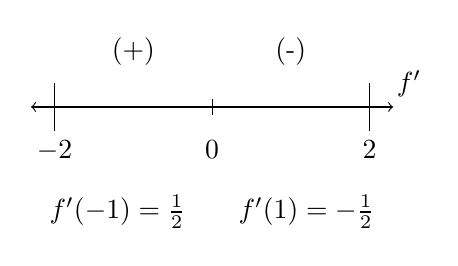
\begin{tikzpicture}

%\draw[help lines] (-2,-2) grid (2,2);

\draw [<->] (-2.3,0) -- (2.3,0);
\draw (-2,0.3) -- (-2,-0.3);
\draw (0,0.1) -- (0,-0.1);
\draw (2,0.3) -- (2,-0.3);

\draw (-2,-0.3)node[below]{$-2$};
\draw (0,-0.3)node[below]{$0$};
\draw (2,-0.3)node[below]{$2$};
\draw (-1.2,-1)node[below]{$f'(-1) = \frac{1}{2}$};
\draw (1.2,-1)node[below]{$f'(1) = - \frac{1}{2}$};
\draw (-1,1)node[below]{(+)};
\draw (1,1)node[below]{(-)};
\draw (2.5,0)node[above]{$f'$};


\end{tikzpicture}
\end{image}
\end{center}

%%%%%%%%%%%%%%%%%%%%%%%%%%%%%%%%%%%%%%%%%%%%%%%%%%%%%%%%%%%%%%%%%%%%%%%%%%%%%%%%%%%%%%%%

		Thus, $f'$ is positive on the interval $(-2,0)$ and negative on $(0,2)$, and therefore $f$ is increasing on $(-2,0)$ and decreasing on $(0,2)$.  
		\end{freeResponse}
	%part d	
	\item  Local extrema (and check your answers with both the first and second derivative tests)
	
		\begin{freeResponse}
		At $x=0$, $f'$ changes sign from positive to negative.  Thus $f$ goes from increasing to decreasing, and therefore by the first derivative test $x=0$ is a local maximum of $f$.  
		
		For the second derivative test, we have that
		$$ f''(0) = \frac{6(0)^2 - 2}{(1+0^2)^3} = \frac{-2}{1} = -2 < 0 $$
		and thus we again conclude that $x=0$ is a local maximum of $f$.
		\end{freeResponse}
	%part e	
	\item  Intervals of concavity
	
		\begin{freeResponse}
		To find points were $f''$ may change signs, we need to find where $f''(x)=0$ or $f''(x)$ does not exist.  $f''(x)$ exists everywhere in our domain so we are only looking for where $f''(x)=0$.  So we solve
		\begin{align*}
  		& \frac{6{{x}^{2}}-2}{{{(1+{{x}^{2}})}^{3}}}=0 \\ 
 		& 6{{x}^{2}}-2=0 \\ 
 		& {{x}^{2}}=\frac{2}{6} \\ 
 		& x=\pm \frac{1}{\sqrt{3}} \\ 
		\end{align*}
		
		We can determine intervals of concavity two ways:\\\\
		First, since the denominator of $f''$ is always positive, $f''$ has the same sign as the numerator.  The factors of the numerator are $\left(x- \frac{1}{\sqrt{3}} \right) \left(x+ \frac{1}{\sqrt{3}} \right) $.  When $x>\frac{1}{\sqrt{3}}$, both factors are positive and $f''>0$.  When $x<-\frac{1}{\sqrt{3}}$, both factors are negative and $f''>0$.  When $-\frac{1}{\sqrt{3}}<x<\frac{1}{\sqrt{3}}$, one factor is negative and the other is positive so $f''<0$. Thus, $f$ is concave down on $\left( - \frac{1}{\sqrt{3}}, \frac{1}{\sqrt{3}} \right)$ and concave up on $\left( -2, - \frac{1}{\sqrt{3}} \right)$ and $ \left( \frac{1}{\sqrt{3}}, 2 \right)$\\\\
		
		The other way we go about this is using test points:
		Picking test points of $-1, 0, $ and $1$, we have that
		\begin{align*}
		& f''(-1) = \frac{6-2}{2^3} = \frac{4}{8} > 0 \\
		& f''(0) = \frac{0-2}{1^3} = \frac{-2}{1} < 0 \\
		& f''(1) = \frac{6-2}{2^3} = \frac{4}{8} > 0 \\
		\end{align*}
		So we have the following picture:
		
%%%%%%%%%%%%%%%%%%%%%%%%%%%%%%%%%%%%%%%%%%%%%%%%%%%%%%%%%%%%%%%%%%%%%%%%%%%%%%%%%%%%%%
		
\begin{center}
\begin{image}
\begin{tikzpicture}

%\draw[help lines] (-2,-2) grid (2,2);

\draw [<->] (-4.6,0) -- (4.6,0);
\draw (-4,0.3) -- (-4,-0.3);
\draw (-1.1547,0.1) -- (-1.1547,-0.1);
\draw (1.1547,0.1) -- (1.1547,-0.1);
\draw (4,0.3) -- (4,-0.3);

\draw (-4,-0.3)node[below]{$-2$};
\draw (-1.1547,-0.3)node[below]{$- \frac{1}{\sqrt{3}}$};
\draw (1.1547,-0.3)node[below]{$\frac{1}{\sqrt{3}}$};
\draw (4,-0.3)node[below]{$2$};
\draw (-3,-2)node[below]{$f''(-1) = \frac{1}{2}$};
\draw (0,-2.2)node[below]{$f''(0) = -2$};
\draw (3,-2)node[below]{$f''(1) = \frac{1}{2}$};
\draw (-2.5,1)node[below]{(+)};
\draw (0,1)node[below]{(-)};
\draw (2.5,1)node[below]{(+)};
\draw (5,0)node[above]{$f''$};


\end{tikzpicture}
\end{image}
\end{center}

%%%%%%%%%%%%%%%%%%%%%%%%%%%%%%%%%%%%%%%%%%%%%%%%%%%%%%%%%%%%%%%%%%%%%%%%%%%%%%%%%%%%%%%%

		
		
		Thus, $f$ is concave down on $\left( - \frac{1}{\sqrt{3}}, \frac{1}{\sqrt{3}} \right)$ and concave up on \\ 
		$\left( -2, - \frac{1}{\sqrt{3}} \right)$ and $\left( \frac{1}{\sqrt{3}}, 2 \right)$
		\end{freeResponse}
	%part f	
	\item  Inflection points
	
		\begin{freeResponse}
		To find the inflection points, we need to find where $f''(x)=0$ or $f''(x)$ does not exist, \dfn{and} where $f''$changes sign.  We found these values in part (e):
		\begin{align*}
 		 & f\left( \frac{1}{\sqrt{3}} \right)=\frac{3}{4} \\ 
 		& f\left( -\frac{1}{\sqrt{3}} \right)=\frac{3}{4} \\ 
		\end{align*}  
		So our inflection points are: $\left( -\frac{1}{\sqrt{3}},\frac{3}{4} \right),\left( \frac{1}{\sqrt{3}},\frac{3}{4} \right)$
		\end{freeResponse}
	%g	
	\item  Absolute extrema
	
		\begin{freeResponse}
		We need to check the critical points of $f$ and the endpoints of the interval:
		\begin{align*}
  		& f(-2)=\frac{1}{5} \\ 
 		& f(0)=1 \\ 
 		& f(2)=\frac{1}{5} \\ 
		\end{align*}
		So the absolute maximum value of $f$ on $[-2,2]$ is $f(0)=1$.  Both $f(-2)=\frac{1}{5}$ and $f(2)=\frac{1}{5}$ are the absolute minimum values of $f$ on $[-2,2]$.
		
		The graph of the function looks like:
		
%%%%%%%%%%%%%%%%%%%%%%%%%%%%%%%%%%%%%%%%%%%%%%%%%%%%%%%%%%%%%%%%%%%%%%%%%%%%%%%%%%%%%%%%
\begin{center}
\begin{image}
\begin{tikzpicture}[xscale=2,yscale=2]

\draw [<->] (0,2) -- (0,0) -- (3,0);
\draw [<->] (0,-1) -- (0,0) -- (-3,0);
\draw[red, ultra thick, domain=-2:2] plot (\x, {1/(1+(\x)^2)});
\draw (-2,0.1) -- (-2,-0.1);
\draw (2,0.1) -- (2,-0.1);
\draw (-2,-0.3)node[below]{$-2$};
\draw (2,-0.3)node[below]{$2$};
\draw (-0.57735,0.1) -- (-0.57735,-0.1);
\draw (0.57735,0.1) -- (0.57735,-0.1);
\draw (-0.57735,-0.2)node[below]{$- \frac{1}{\sqrt{3}}$};
\draw (0.57735,-0.2)node[below]{$\frac{1}{\sqrt{3}}$};

\end{tikzpicture}
\end{image}
\end{center}
%%%%%%%%%%%%%%%%%%%%%%%%%%%%%%%%%%%%%%%%%%%%%%%%%%%%%%%%%%%%%%%%%%%%%%%%%%%%%%%%%%%%%%%%


		\end{freeResponse}
	
	\end{enumerate}
		
\end{problem}



%problem4

\begin{problem}

  \begin{enumerate}
  %part a
    \item
      The (entire) graph of a function $f$ is shown in the figure below.
      \begin{image}
        \includegraphics[scale = 0.3]{figure3.png}
      \end{image}
      \begin{enumerate}
      	%part i
        \item
          Find the $x$-coordinates of all critical points of $f$ (or write NONE).
          \begin{freeResponse}
            $f$ has a critical point at $x = 0$ since $f'(0) = 0$

            $x = 1$ is a critical point since $f'(1)$ DNE.

            $x = 3$ is a critical point since $f'(3)$ DNE.
          \end{freeResponse}
	%part ii
        \item
          Find the $x$-coordinates of all local minima of $f$ (or write NONE).
        
          \begin{freeResponse} 
           By first derivative test there is a local minimum at $x=3$
          \end{freeResponse}

        \item
          Find all values of $x$ at which $f$ attains its global minimum (or write NONE).
          \begin{freeResponse}
            $f(3) = 0$ and $\lim_{x \to -1^+} f(x) = -2$ (but $f(-2)$ DNE) imply $f$ has no global minimum
          \end{freeResponse}

        \item
          Find the interval (or intervals) on which the \emph{derivative of $f$} is increasing.
          \begin{freeResponse}
            $f'$ is increasing  on (0,1): $f$ is concave up on this interval
          \end{freeResponse}

      \end{enumerate}

    \item
      The figure below shows the graphs of $f$, $f'$, and $f''$.
      Which curve is which?
      \begin{image}
        \includegraphics[scale = 0.3]{figure2.png}
      \end{image}
      \begin{freeResponse}
        Graph A is $f$, Graph B is $f'$ and Graph C is $f''$.
      \end{freeResponse}


  \end{enumerate}
\end{problem}

	
	
%problem5	
\begin{problem}
Given the graph of $h'$, sketch a graph of $h$ and $h''$ on the same set of axis.
      \begin{image}
        \includegraphics[scale = 0.6]{figure1.png}
      \end{image}



\begin{freeResponse} \hfil


      \begin{image}
        \includegraphics[scale = 0.5]{figure7.png}
      \end{image}	
				
				
To sketch $h''$ from $h'$, we need to think back to section 3.2.  It might be easier for you to think of $h'=g$ and $h''=g'$.  We're really just sketching a graph of the derivative from the graph of its function.  \\

We need to recall when the graph of:\\
$h'=g$ is increasing, $h''=g'$ is positive\\
$h'=g$ is decreasing, $h''=g'$ is negative\\
$h'=g$ has a local maxima or minima, $h''=g'=0$\\
$h'=g$ has an inflection point, $h''=g'$ has a local maxima or minima\\
$h'=g$ is concave up, $h''=g'$ is increasing\\
$h'=g$ is concave down, $h''=g'$ is decreasing\\

$\implies$
The graph of $h''=g$ is/has:
Positive slope on the intervals $(-\infty,-1.5)$ and $(2,\infty)$\\
Negative slope on the interval $(-1.5,2)$\\
Local maximum at $x=-1.5$, local minimum at $x=2$\\
Inflection point at $x=0$\\
Concave down on the interval $(-\infty,0)$\\
Concave up on the interval $(0,\infty)$\\\\

To sketch $h$ from $h'$, we are using the same information, but in reverse.  \\\\
The graph of $h$ is/has:\\
Positive slope on the intervals $(-\infty,2)$ and $(5.5,\infty)$\\
Negative slope on the interval $(2,5.5)$\\
Local maximum at $x=2$\\
Inflection points at $x=-3,0,4$\\
Concave down on the intervals  $(-\infty,-3)$ and $(0,3.7)$\\
Concave up on the intervals $(-3,0)$ and $(3.7,\infty)$


		
						
\end{freeResponse}
\end{problem}

%problem6
\begin{problem}
Give an example or sketch of a function that is continuous on $(-\infty,\infty)$ and satisfies given properies.  If such a function does not exist, explain why.
\begin{enumerate}
	\item A function $f$ is concave up and negative everywhere.
	\begin{freeResponse}
	This is not possible.  If a function is always concave up then at some point, the function must cross the $x$-axis and become positive.  See the three example figures below.
	      \begin{image}
        \includegraphics[scale = 0.5]{figure8.png}
      \end{image}	
			
	\end{freeResponse}
	\item A function $f$ is decreasing and concave up everywhere.
	\begin{freeResponse}
	This is possible.  See figure B above.
	\end{freeResponse}	
	\item A function $s$ has exactly 3 local extrema and four inflection points.
		\begin{freeResponse}
	This is possible.  See the figure below.  The graph of $s$ has inflection points at $a,b,c,d$ and local extrema at $e,f,g$.
		      \begin{image}
        \includegraphics[scale = 0.5]{figure9.png}
      \end{image}	
	\end{freeResponse}	
	\item A function $f$ has exactly 2 zeros and one local extrema.
  	  		\begin{freeResponse}
	This is possible.  See the figures below for examples.
		      \begin{image}
        \includegraphics[scale = 0.5]{figure10.png}
      \end{image}	
      	\end{freeResponse}	

\end{enumerate}



\end{problem}



%problem7
\begin{problem}
Consider the parabola $f(x)=ax^2+bx+c$ where $a,b,c$ are constants.  For what values of $a,b,c$ is $f$ concave up?  For what values of $a,b,c$ is $f$ concave down?				
\begin{freeResponse}
\begin{align*}
f'(x)&=2ax+b\\
f''(x)&=2a
\end{align*}
$\implies$ the sign of $a$ will determine is $f$ is concave up or down.  When $a<0$, $f$ is concave down.  When $a>0$, $f$ is concave up.  Note: If $a=0$, $f$ has no concavity because it is a linear function.


				
\end{freeResponse}
				
\end{problem}	


%problem8
\begin{problem}
Locate the critical points and use the second derivative test to determine whether they correspond to local maxima or local minima.
$f(x)=(x+c)^4$ where $c$ is a positive constant 

\begin{freeResponse}

$$f'(x)=4(x+c)^3, f''(x)=12(x+c)^2$$

To find the critical points: $f'(x)=0=4(x+c)^3$.  This occurs when $x=-c$
 
Using the second derivative test: $f''(-c)=12(-c+c)^2=0$.  The second derivative test was inconclusive so we need to use the first derivative test.

Making a sign chart we see that if we plug something a little less than $-c$ into $f'$, we'll get a negative number.  If we plug something a little greater than $-c$ into $f'$, we'll get a positive number. 

      \begin{image}
        \includegraphics[scale = 0.3]{figure4.png}
             \end{image}

Therefore, there is a local minimum at $x=-c$.  This is also a global minimum.

\end{freeResponse}
\end{problem}







\end{document} 


















